\documentclass[12pt]{article}
\usepackage[english]{babel}
\usepackage[utf8x]{inputenc}
\usepackage{amsmath}
\usepackage{tablefootnote}
\usepackage{amssymb}
\usepackage{graphicx}
\usepackage{float}
\usepackage[colorinlistoftodos]{todonotes}
\usepackage{geometry}
\usepackage{booktabs}
\usepackage{siunitx}
\usepackage{tabularx}
\usepackage{placeins}
\usepackage{booktabs}
\usepackage{xcolor}
\usepackage{colortbl}
\usepackage{multirow}
\usepackage[acronym]{glossaries}
\usepackage{indentfirst}
\usepackage{algorithm}
\usepackage{algorithmic}
\usepackage{algpseudocode}

\usepackage{array}
 

\usepackage[
  backend=biber,
  style=alphabetic,
  maxbibnames=10,
  minalphanames=2,
  citestyle=authoryear-comp, 
  sorting=nyt
]{biblatex}
\addbibresource{biblio.bib}

\usepackage[colorlinks=true,linkcolor=blue,citecolor=blue,urlcolor=blue]{hyperref}
\hypersetup{
    colorlinks=true,
    linkcolor=blue,
    citecolor=blue,
    urlcolor=blue
}



\geometry{letterpaper, margin=0.7in}
\usepackage{subcaption}



\makeglossaries

\newglossaryentry{latex}
{
        name=latex,
        description={Is a mark up language specially suited for 
scientific documents}
}

\newacronym{bhs}{BHS}{Baggage Handling System}
\newacronym{adp}{ADP}{Groupe Aéroports de Paris}
\newacronym{rf}{RF}{Random Forest}
\newacronym{xgboost}{XGBoost}{Extreme Gradient Boosting}
\newacronym{lgbm}{LGBM}{Light Gradient Boosting Machine}
\newacronym{dgo}{DGO}{Direction Générale des Opérations}
\newacronym{eb1}{EB1}{registration banks}
\newacronym{ebs}{EBS}{bagage stocker}
\newacronym{etp}{ETP}{primary sorting}
\newacronym{enl}{ENL}{manual inspection stations}
\newacronym{ei1}{EI1}{registration banks}
\newacronym{edc}{EDC}{correspondence deposits}
\newacronym{ets}{ETs}{transit zone}
\newacronym{etb}{ETB}{final sorting}
\newacronym{ejt}{EJT}{piers}
\newacronym{f}{TBF}{Bagage handling system F}
\newacronym{m}{TBM}{Bagage handling system M}
\newacronym{e}{TBE}{Bagage handling system E}
\newacronym{mbis}{Mbis}{Stocker M}
\newacronym{aobt}{AOBT}{Actual outbound time}
\newacronym{sobt}{SOBT}{Scheduled outbound time}
\newacronym{cdgb}{CDGB}{Charles de Gaulle Baggage department}









\begin{document}
\newcommand{\HRule}{\rule{\linewidth}{0.5mm}} 

\thispagestyle{empty}
\hspace{10cm}
\begin{center}

\vfill
\begin{center}
  
\includegraphics[width=0.38\textwidth]{AMU logo.png}
  \hfill
  
\includegraphics[width=0.43\textwidth]{logo_Groupe_ADP.jpg}
\end{center}
\vfill


\vspace{0.5cm}
%\textsc{\huge Apprenticeship Report}
%\vspace{3cm}

\HRule \\[0.4cm]
{ \huge \textbf{Forecasting mishandled baggage with machine learning models} \\[0.5cm] 
Paris-Charles de Gaulle airport
}\\[0.4cm]
\HRule \\[8cm]
\begin{minipage}[t]{0.7\textwidth}
	\begin{itemize}
    \item[\emph{Author:}] \textbf{Olivier JAYLET}
    \item[\emph{Program:}] \textbf{M.Sc. Econometrics, Big Data and statistics}
    \item[\emph{Supervisor:}] \textbf{Florian BERTOSIO}
    \item[\emph{Submission:}] \textbf{August 30, 2024}
	\end{itemize}
\end{minipage}

\end{center}

















\newpage

\renewcommand{\contentsname}{Table of contents}\tableofcontents

\newpage
\listoffigures
\listoftables
\newpage


\section*{Introduction}
\addcontentsline{toc}{section}{Introduction}
\label{introduction}

Paris-Charles de Gaulle airport, one of Europe's leading air transport hubs, welcomes millions of passengers from all over the world every year. Passenger satisfaction is a top priority for airport operators, who are constantly striving to improve the efficiency and quality of the services they offer.  \hfill \break


A large part of the logistics involves sorting and routing bagages. For safety purposes, any baggage exceeding 115 centimeters (height + width + depth) must be checked in with the airline. For this reason, airlines and airports must cooperate to ensure the smooth transit of bagages from check-in desks to aircraft holds. Moreover, when a passenger transits through a third-party airport on a journey and changes planes the baggage must also follow them. \hfill \break


In this context, Groupe \acrshort{adp} and Air France are working together to ensure the best possible routing of baggages. In 2007, to automate the sorting and routing of baggages  \acrshort{adp} built one of the largest \acrlong{bhs}\footnote{type of conveyor system installed in airports that transports checked luggage from ticket counters to areas where the bags can be loaded onto airplanes} in Europe at Paris-Charles de Gaulle airport. This \acrshort{bhs}, built in collaboration with Siemens, uses various types of sensors to detect, locate, monitor and route baggages through the different sections of the \acrshort{bhs}. Thanks to these sensors, we are able to collect a large amount of data and thus use them to analyse, understand and optimise baggage flow.  \hfill \break

The ability to analyse the reasons why a baggage misses it's flight is of upmost financial importance. A mishandled bag will cost \acrshort{adp} or the airline an average of 300 euros. The objective for \acrshort{adp} is to reduce the number of mishandled baggages and be able to quantify and identify why or how a baggage was mishandled. \hfill \break

My aim is to train and test several classification machine learning models to forecast if a baggage will be mishandled once it enters in \acrshort{adp}'s baggage handling facilities. Another model trying to predict the handling time in the \acrshort{bhs}, referred to henceforth as path duration is being developed in parallel\footnote{by colleague, Miracle Vodoumbo}, I included this variable\footnote{the path duration is highly correlated with the probability of mishandling a baggage (see \autoref{subsubsec:Path duration}), adding it to the model gives a very important information.} in my models assuming we will be able to estimate it for each baggage when entering the \acrshort{bhs}.  \hfill \break

Firstly, a bunch of descriptive statistics were analysed to estimate the usefulness of variables in predicting mishandled bags. \hfill \break
\noindent Secondly, a logistic regression was performed as a benchmark model to compare with a \acrlong{rf}, an \acrlong{xgboost} and a \acrlong{lgbm}. Having a higly imblanced dataset\footnote{\autoref{section:Imbalanced dataset issue}}, probabilities were calibrated with methods such as platt scaling\footnote{\autoref{Platt scaling}} and isotonic regression\footnote{\autoref{Isotonic regression}}. \hfill \break 
\noindent Finally, noises were added in the bag path duration variable according to the current errors of the bag path duration model estimations. Adding noise and randomness to this variable is essential to check whether or not the predictions of mishandled bags lose much accuracy.

% Finally, noise was added to the path duration variable during the training process of each of my models to emulate estimation errors.

%The aim of this research is to provide airport operators with valuable tools and information to better anticipate passenger ground transportation needs, which could help improve the operational efficiency of Paris-Charles de Gaulle airport. 


%Dans les chapitres suivants, nous allons présenter l’environnement de travail puis nous décrirons la problématique du sujet. Ensuite, nous ferons un état de l’art des différentes méthodes d’apprentissage utilisées pour la prévision de flux. 
%Pour finir, nous examinerons en détail l’approche retenue, les résultats obtenus ainsi que les axes d’amélioration possibles.
\newpage
\section{Data and management team}

\begin{figure}[h]
    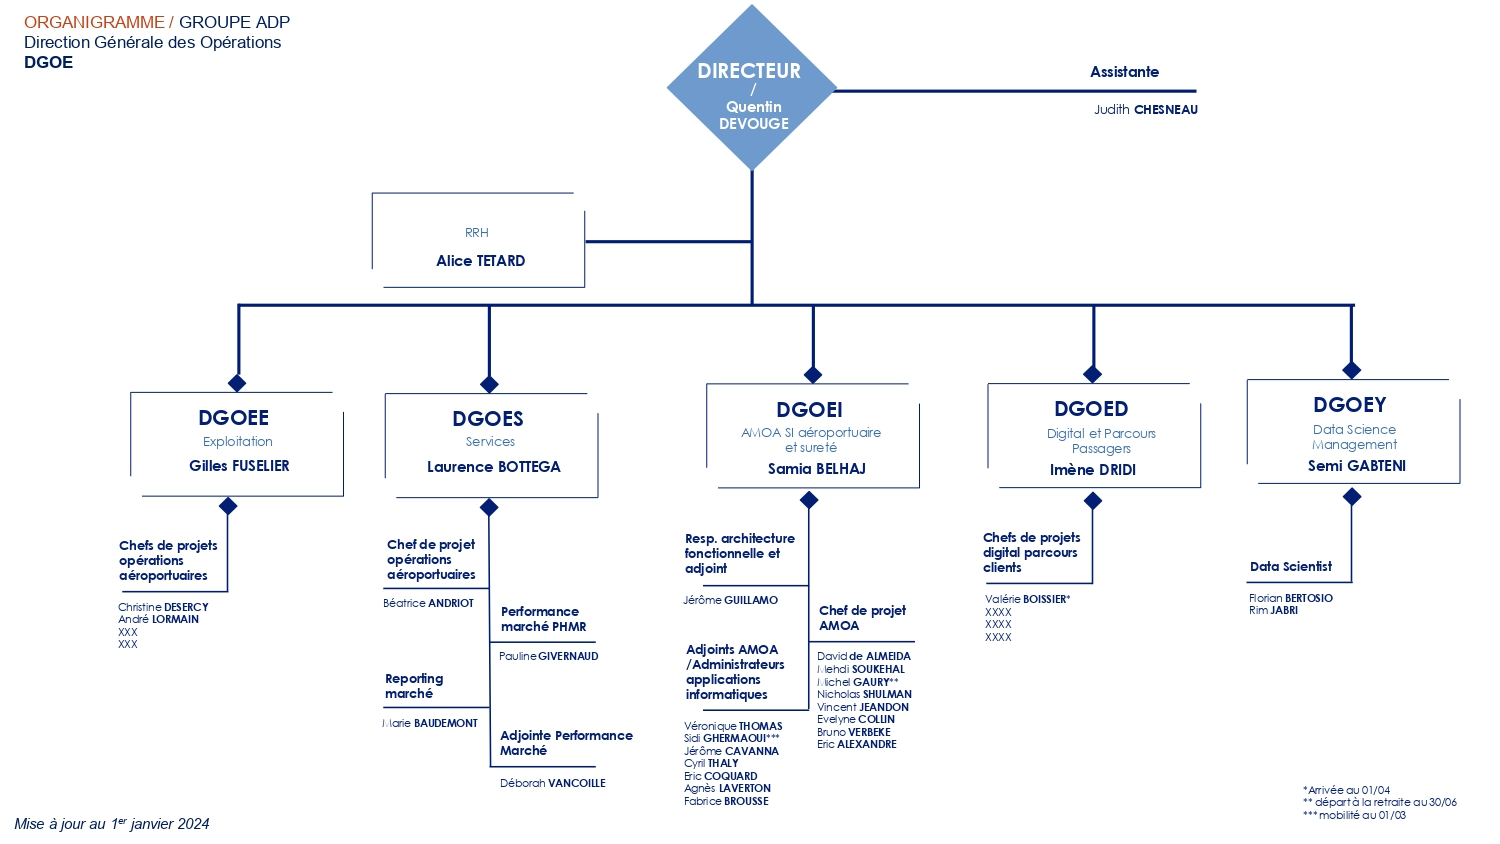
\includegraphics[width=1\textwidth]{organigramme_DGO.jpg}\\
    \caption{Organization chart : \acrshort{dgo}}
\end{figure}
\FloatBarrier


\newpage
\section{Related work}

There is literature on the logistics of baggage sorting and \acrlong{bhs}, but only one study has been carried out that is closely related to my topic of failed baggage.
\cite{MishandledBgas} trained and tested a \acrlong{lgbm} to predict for each bag a probability of being a mishandled baggage. The aim of this study is to identify "at-risk" baggage. A logistic model was also tested, serving as a benchmark model. \hfill \break 
\noindent This study was carried out in collaboration with an airline, and the model developed predicts probabilities only for baggage in transit. Consequently, none of the data used comes from the \acrshort{bhs} , but only from data known by the airline, which therefore offers fewer subtleties. Finally, oversampling\footnote{method used to address class imbalanced by increasing the number of instances in the minority class.} was used to overcome the problem of unbalanced dataset, without attempting to calibrate the model beforehand. Therefore, the model was trained with generated data. \hfill \break
\noindent The final model with the best results has a recall of 0.565, a Precision score of 0.506 and an F1 score of 0.534 \footnote{see \autoref{equation:Recall} \autoref{equation:Precision} \autoref{equation:F1-score}}.

In the same purpose of avoiding mishandling bags, \cite{ForecastingFramework} predicts the probability of a bag to recirculate at least once in the \acrlong{bhs}. Using sensors data within the \acrshort{bhs}, the prediction model achieved a precision of 0.956 and a recall of 0.033 for detecting behavior. When excluding bags that had recirculated before, the recall improved to 0.153 abd tge precision dropped to 0.764. Even tho the model wasn't trained in the same \acrshort{bhs}, it is an interesting approach, as recirculating is a cause of longer processing time by \acrshort{ADP}, being able to predict whether or not a bag will make another loop would most probably help to improve mishandling predictive models. \hfill \break 


\cite{SchedulingBGF}
\cite{ImprovementofaSortationSystem}
\cite{Pillière}

\newpage


\section{Data and Descriptive statistics}

A large part of my apprenticeship was spent studying the data. The \acrlong{bhs} being very complex, it was not trivial to understand the data. A lot of primary intuition wasn't enough to be able to model baggage paths. Numerous discussions with the data-scientists of my team, as well as with the professionals in the \acrshort{cdgb} department\footnote{department in charge of baggage logistic} helped me to understand all biases and differences in between data and actual processes. Those discussions and the analysis of descriptive statistics gave me some idea on how to solve model the \acrshort{bhs}, and what data I could create or modify for some computing and modelling optimisations. 

In this section, I'll first introduce you the table of original data. Then we will talk about the most relevant descriptive statistics I made, and the feature engineering methods it leaded to.


\subsection{Original dataset}

Our dataset come from several databases. The first called \textit{fact\_paths} contains data of each bagage paths. These datas are extracted daily through a pipeline sending requests to the software package used by \acrshort{bhs} managers and analysts. In this table, we access the data of each baggage journey (path) in the \acrshort{bhs}, from the injection of the baggage into the sorter until its extraction.
The second database, \textit{Saria\_info\_vol} contains flight information such as airlines, departure times, departure and destination airports, etc. Thanks to a unique identifier, we are able to link baggage trajectories to information on their feeder and transport flights\footnote{explication apport/emport}. \hfill \break
\indent The \autoref{tab:variables} list all data we managed to join. As the aim of this project is to predict the status of baggage when it leaves the \acrshort{bhs}, we need to use data available before it enters the sorter. For example, \acrshort{aobt} is a variable available after baggage exits the \acrshort{bhs}. Including it in the model means giving a variable that directly indicates whether or not the baggage is missed. If the flight takeoff before bag leaves the sorter, then the bag was obviously mishandled.\\ 
The number of additional loops around the primary belt is also a variable known during the sorting process. This data depends on a rerouting algorithm which makes bags run another loop according to flow and time difference in between bags. As we don't have access to this algorithm yet and can't predict it, I didn't include \textit{recirc\_gb\_cnt} in models.


% \noindent The variable \textit{total\_path\_duration\_no\_stock} cannot be known before the bag injection in the sorter. However, as we'll see in descriptive statistics (see \autoref{subsubsec:Path duration}), path duration in the sorter is highly correlated with the probability of failed bag. As explained in the introduction, Data and management team is currently training some models to predict the duration of bags before it enters the sorter. In \autoref{subsubsec:Path duration} I explain the methodology to add noise to path duration and therefore transform path duration as a proxy.

\begin{table}[ht]
    \centering
    \caption{Dictionary of Variables}
    \label{tab:variables}
    \begin{tabularx}{\textwidth}{lclX}
        \toprule
        \textbf{Variable} & \textbf{Type} & \textbf{Description} \\
        \midrule
        id\_bag\_trajet & int64 & Bag path id. \\
        input\_date & datetime & Date and time baggage entered sorter. \\
        input\_module & String & Bag input module. \\
        input\_position & String & Sub-system at which baggage enters sorter. \\
        input\_status & String & Bag status on entering the sorter. \\
        input\_outbnd\_flt\_dhc & Float & Date and time of flight known when bag enters sorter. \\
        output\_module & String & Bag exit module in the sorter. \\
        output\_position & String & Bag exit sub-system. \\
        inbnd\_flt\_hab & datetime &  Date and time of outbound aircarft.\\
        input\_ICT\_BHS & float64 & Time in minutes between baggage injection and the SOBT. \\
        count\_EBS & int64 & Number of time the bag was stored in \acrshort{ebs} \\
        count\_TBS & int64 & Number of time the bag was stored in TBS \\
        has\_flight\_changed & bool & The outbound flight has changed during the bag path. \\
        total\_path\_duration\_no\_stock & float64 & Total baggage transit time in minutes, excluding storage \\
        path\_length & int64 & Number of times the bag was detected inside the sorter. \\
        recirc\_gb\_cnt & int64 & Number of additional loop on the primary belt. \\
        %SIBT & datetime & Scheduled inbound time of the intake aircraft. \\
        %AIBT & datetime & Actual inbound time of the intake aircraft. \\
        geographic\_origin & String & Inbound flight origin. \\
        geographic\_dest & String & Outbound flight destination. \\
        SOBT & datetime & Scheduled outbound time of the outbound aircraft. \\
        AOBT & datetime & Actual outbound time of the outbound aircraft. \\
        is\_failed & bool & Has the baggage been failed ? (Variable to predict) \\
        
        \bottomrule
    \end{tabularx}
\end{table}
\FloatBarrier







\newpage
\subsection{Descriptive Statistics}

METTRE LES DATES DES DONNEES

\subsubsection{Seasonality}
The sorter opening at around 5 a.m. until 11 p.m. every day of the week, the first intuition we might have about mishandled baggage is the presence of seasonality.
For these reasons, it is important to visualize the evolution of missed baggage over time. \autoref{fig:Average number and percentage of failed bags each days of the week}
shows the evolution by day of the week of the number of missed bags, as well as the percentage of
rates

\begin{figure}[h]
    \centering
    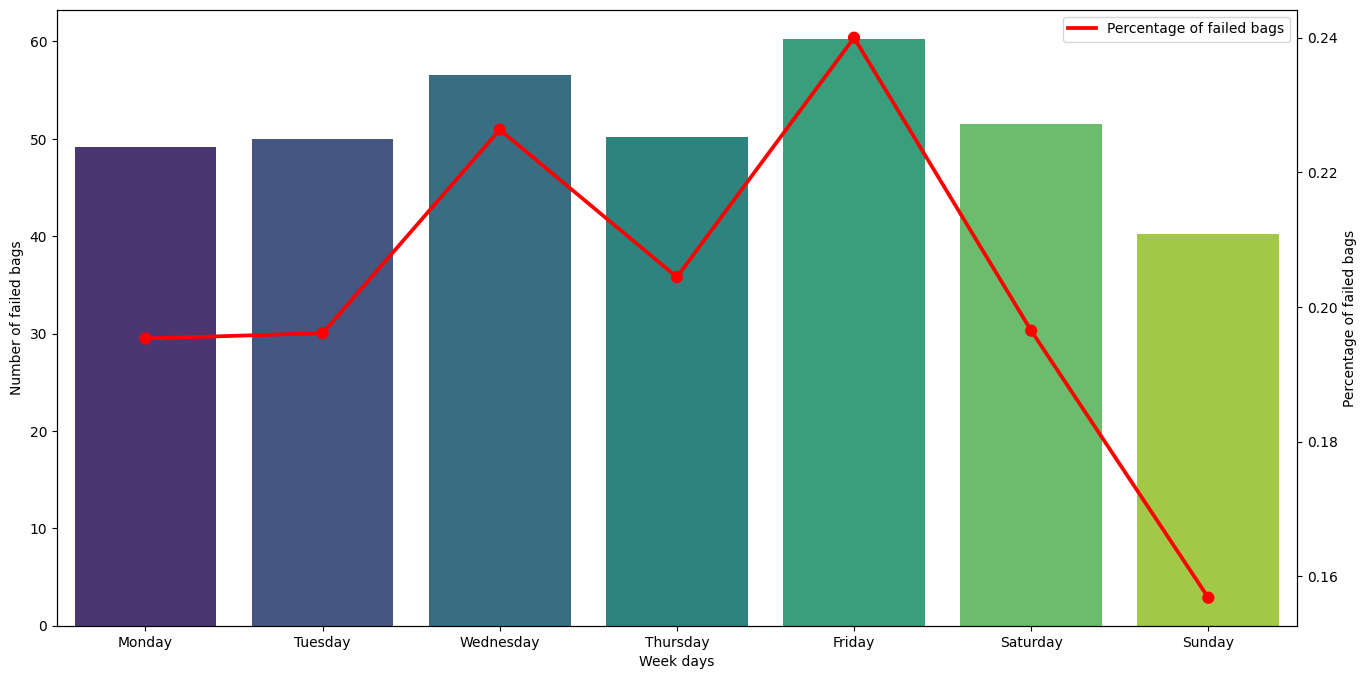
\includegraphics[width=0.9\textwidth]{Number and percentage of failed bags within a week.png}\\
    \caption{Average number and percentage of failed bags each days of the week}
    \label{fig:Average number and percentage of failed bags each days of the week}
\end{figure}
\FloatBarrier

It's straight forward to see that failed bags volumes are changing according to the week days. Weekends seem to be less problematic, both in terms of volume and percentage. Intuitively, we might have expected weekends to be more complicated (given the greater number of passengers during weekends). Perhaps because logistics teams are more numerous to better manage the heavy flows at weekends, therefore it can be more difficult to avoid failed bags during the week, with teams that could be smaller.

To analyse more in detail failed bags pattern with regard to time, the Figure \ref{fig:Average number and percentage of failed bags each 30 minute of a day} displays the average number and percentage of failed bags for each 30 minute of a day.

\begin{figure}[h]
    \centering
    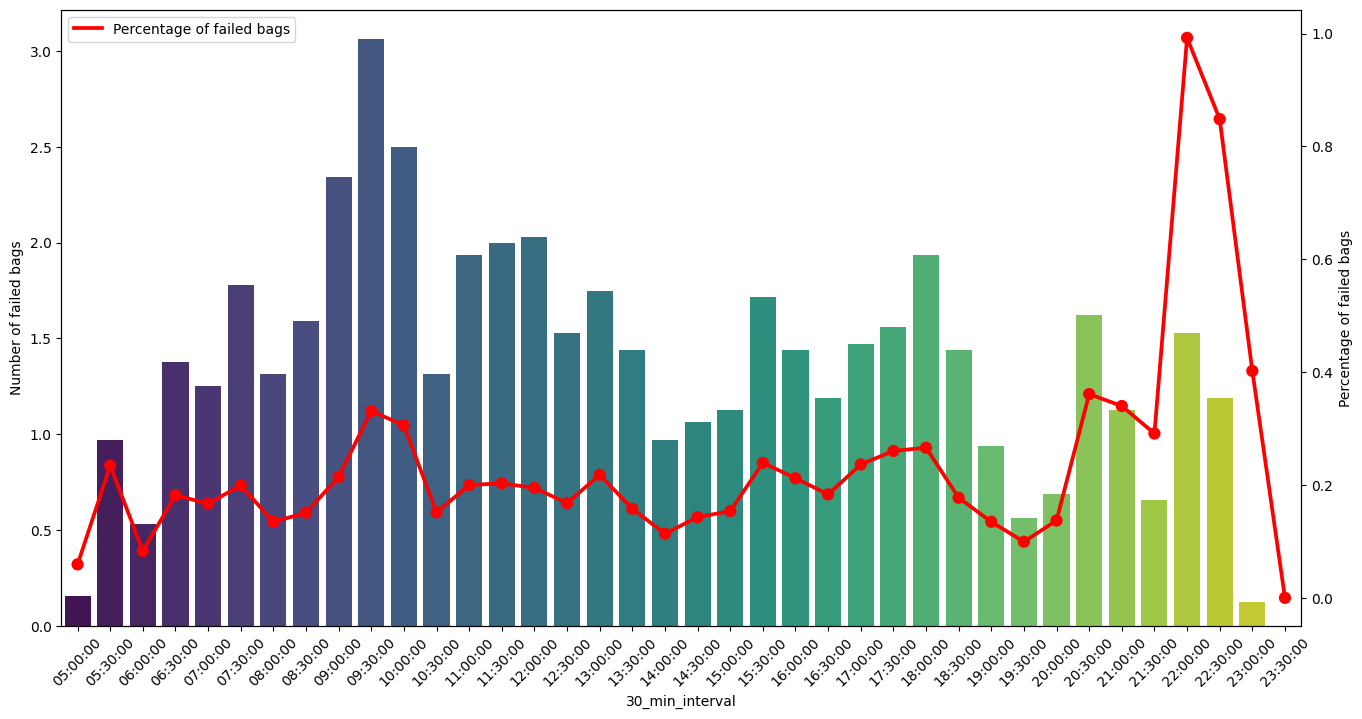
\includegraphics[width=0.9\textwidth]{Number and percentage of failed bags within a day.png}\\
    \caption{Average number and percentage of failed bags each 30 minute of a day}
    \label{fig:Average number and percentage of failed bags each 30 minute of a day}
\end{figure}
\FloatBarrier

It turns out there is a peak of failed bags at around 9am in the morning. This could be explained by the large number of flight departure in the morning. We can also see that the percentage of failed bags is stable until around 9pm, where it suddently increase to get its peak. This is most probably dur to two reasons. Firstly, handlers feed the sorter at the end of the day with a lot of bags which were failed and which will get stored into a stocker during the night. Those bags are already failed before entering the sorter and we have to be aware of this bias while interpreting models results. Moreover, there is less flight at this end of the day, so the number of actual traveling bags is lower while the number of failed bags (when being injected) is higher.

\indent Thanks to those figures, we can be sure there are some seasonal effects on the probability to fail a bag. To model it and capture seasonal effects, a special encoding process can be applied as day and hours are cyclical features. Following the method of sin and cosines (\cite{HarrisonPim}) seems to be a great strategy as it encodes minute of the day by taking auto correlation in between minutes that might exist.
\noindent The sinus and cosines transformation are defined as follow : 
\begin{equation}
f(x) = \sin\left(\frac{2\pi x}{\text{period}}\right)
\end{equation}

\begin{equation}
g(x) = \cos\left(\frac{2\pi x}{\text{period}}\right)
\end{equation}

\autoref{fig:Cyclical encoding of days and minutes} displays a visualisation of sin and cosine transformations for a few days only. Each days of the week and minutes of the day are smoothly link to each other, and those smoothed lines (especially for minutes of the days) will help the model to recognize seasonal patterns.  

\FloatBarrier

\newpage
\subsubsection{Baggage paths}

The \acrlong{bhs} being very complex, one of the biggest challenge for \acrshort{adp} in their project to reduce the number of mishandled bags and optimize their logistic is to understand how bags travel inside the \acrshort{bhs}. Using bag paths data, we are able to identify problematic paths, which could be a cause of failed bag. As there is a large number of paths\footnote{There are actually more than 700 different observed paths}, we had to analyse some "typical" or usual paths (paths used often).

To better understand the complexity of the \acrshort{bhs}, I will first explain you how bags travels onto sorter and explain what data I decided to use for bag paths. Then I will provide some statistics about those data.

\paragraph{A journey into the \acrshort{bhs}} La logistique de tri bagage est un système très complèxe, au vu de la taille de l'aéroport. Les bagages peuvent provenir soit des vols à l'apport, pour être réacheminé sur des vols à l'emport (ce sont donc des bagages en transit), ou bien injecté directement par les companies aériennes aux banques d'enregistrement. Il existe donc plusieurs points d'entrées et sorties dans l'infrastructure du tri bagage.

Enfin, l'aéroport de Roissy est composé de plusieurs \acrlong{bhs}. Siemens et Braumer sont les deux constructeurs et technologies différentes qui consituent les \acrshort{bhs}. Pour le moment, notre équipe ne détient que les données des \acrshort{bhs} de Siemens, qui sont les modules \acrshort{e}, \acrshort{f} et \acrshort{m}. La \autoref{fig:Simplified diagram of the baggage sorting system "TBE", at the sub-system level} est une simplification du \acrshort{e} à la maille sous-système. Elle permet de visualiser d'un point de vue macro les différents parcours qu'un bagage peut prendre dans le TBE.


\begin{figure}[h]
    \includegraphics[width=0.9\textwidth]{synoptique_simplifié.png}\\
    \caption{Simplified diagram of the baggage sorting system TBE, at the sub-system level}
    \label{fig:Simplified diagram of the baggage sorting system "TBE", at the sub-system level}
\end{figure}
\FloatBarrier
Voici une explication très brève et simplifié d'un parcours bagage dans le \acrshort{bhs} : un bagage peut être injecté dans le \acrshort{e} par trois entrées différentes, les \acrlong{eb1}, les \acrlong{edc}, ou depuis le module F (\acrshort{f}). Une fois qu'un bagage est entré dans le \acrshort{e}, il est acheminé vers le \acrshort{etp} dans lequel il va se diriger vers sa destination. Si le vol du bagage n'est pas encore ouvert, il se dirigera vers un stockeur (\acrshort{mbis} or \acrshort{ebs}) dans lequel il attendra que son vol s'ouvre. Si son vol est déjà ouvert, alors le bagage se dirigera vers les \acrshort{ejt}, où des équipes de manutentionnaire le prendront en main pour l'acheminer du \acrshort{bhs} jusqu'à l'avion.

\paragraph{Simplifiying paths} En réalité, les trajets des bagages au sein du \acrshort{bhs} sont bien plus complexes et présente de nombreuses variante. Pour la modélisation, j'ai décidé de simplifier ces parcours. Au lieu de prendre tous les points de passage d'un parcours, je n'ai utilisé que les points d'entrées et sorties de chaque parcours pour deux granularités différentes. La première est l'échelle module (dans quels modules le bagage entre et sort), la deuxième est l'échelle sous-système (dans quels sous-systèmes le bagages entre et sort). Ces deux granularité donnent effectivement de l'information sur la longueur et difficulté du parcours, sans pour autant prendre toutes les informations du parcours.  





\subsubsection{Paths duration}\label{subsubsec:Paths duration}



\begin{figure}[h]
    \centering
    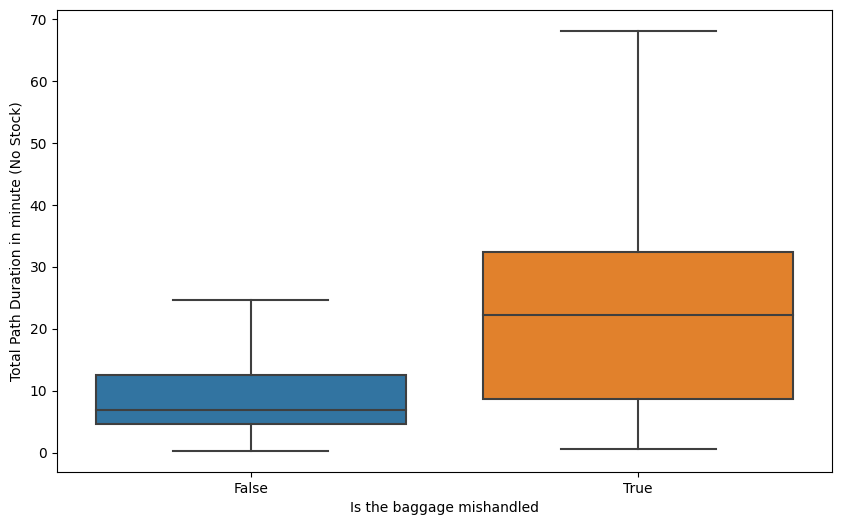
\includegraphics[width=0.6\textwidth]{Boxplot path duration per failed status.png}\\
    \caption{Distribution of paths duration for non-failed and failed bags}
\end{figure}
\FloatBarrier


\paragraph{Past duration time as an indicator} past\_median\_duration\_time


\paragraph{Using model residuals to generate noise}
1 scatter plot et 1 histogramme des résidus de Miracle
explication méthode
plot résidus
lineplot temps réels Vs temps prédis (order ascending)



\subsubsection{Importance of baggage's flow}
past\_nb\_bags
past\_nb\_failed

\subsubsection{Bags input status}
When being injected onto the sorter, bags are classified according to their status. There exists a lot of status, those indicate how the bag should be sorted. Those status are important and can give information to models.

\begin{figure}[h]
    \centering
    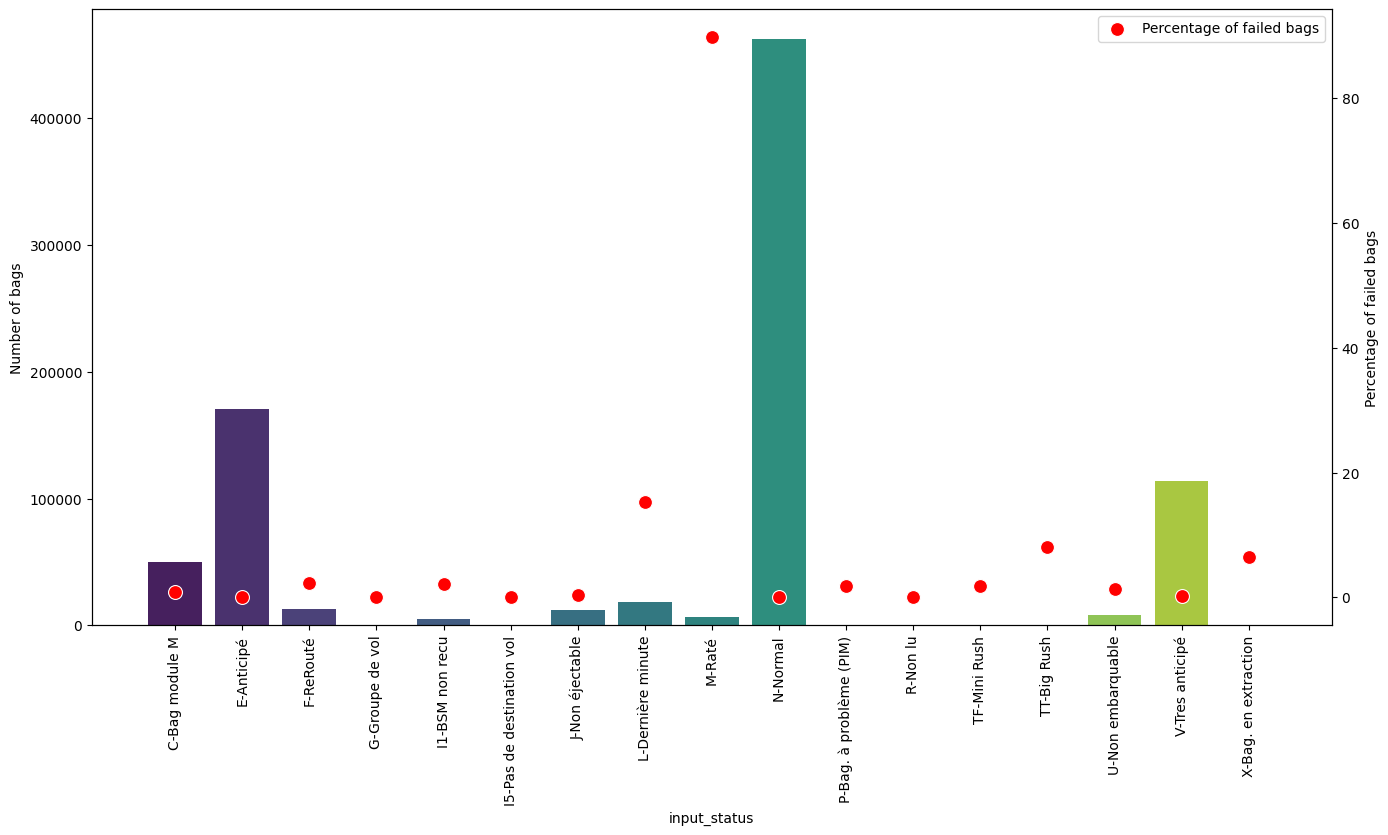
\includegraphics[width=0.9\textwidth]{failed bags per input status.png}\\
    \caption{Number and percentage of failed bags per input status}
    \label{fig:Number and percentage of failed bags per input status}
\end{figure}
\FloatBarrier

All status having different meanings, they also have different frequency. The \textit{normal} status is the most often used and has a low percentage of failed bags. Bags having this status are usually those injected on time in the sorter, when the outbound flight is open to load bags. When a bag is injected earlier and the outbound flight isn't open to load bags, they take the \textit{anticipated} or \textit{very anticipated} status. We could think that injecting a bag much before loading time would be correlated with a lower percentage rate of failed bags. But the \autoref{fig:Number and percentage of failed bags per input status} shows a higher percentage of failed bags for \textit{V-Très anticipé} (very anticipated) bags than \textit{N-Normal} ones. This can be explained by the re-rooting of failed bags. If a flight ends its bag loading process while a bag is still in the sorter, this bag's flight will change (\textit{has\_flight\_changed} will turn \textbf{True}) then its status will change to \textit{V-Très anticipé} (as its unlikely to find another flight soon after missing the previous one) and the bag will be store in a stock to wait.
\noindent The \textit{L-Dernière minute} (last minute) status is given to a bag entering the \acrshort{bhs} knowing there is not much time left. If it manages to exit the \acrshort{bhs} on time, it will be loaded onto the flight with the last minute procedure (manually instead of being put into a container). This status is a very important information for the model as we can see it the category with the higher failed rate (out of \textit{M-Raté}).
\noindent In the aim to model bags output status (failed or not failed), we should carefully consider those \textit{input status} because some of them could make the models to over-fit. For example, \textit{M-Raté} means that the bag is failed when it enters in the \acrshort{bhs}. We should get rid off those kind of bags. 


Finally, here is the list of \textit{input status} we will keep to train and test models : \textit{C-Bag module M, L-Dernière minute, U-Non embarquable, V-Très anticipé, E-Anticipé, P-Bag. à problème (PIM), F-ReRouté, R-Non lu, J-Non éjectable}.

\subsubsection{Minute until flight departure}

Another very important data available is the number of minute before flight departure (input\_ICT\_BHS). Knowing the \textit{SOBT} of a flight and the \textit{input\_date} of a bag, we computed the number of minute in between both. Looking at the \autoref{fig:Minute until flight departure distribution}, it turns out in average, a bag has a bit less than 200 minutes to reach its flight. The distribution looks to be a gaussian distribution, with some extreme value higher than 600 minutes (\textit{V-Très anticipé} bags) and some negative values. Having a negative nume of minute until flight departure mostly mean it's almost impossible to reach its flight on time. However, looking at both distributions of minute until flight departure of failed and non failed bags in the \autoref{fig:Minute until flight departure distribution according to bag status}, we can see a decreasing proportion of non-failed bags from approximately 0 to -100 minutes. It means some bags are still managed even when being pushed onto the \acrshort{bhs} after the schedule outbound time. This is most likely explained by flights delays. Those visualisations give us a first important cause of failed bags, being injected too late in the \acrshort{bhs}.

\begin{figure}[h]
    \centering
    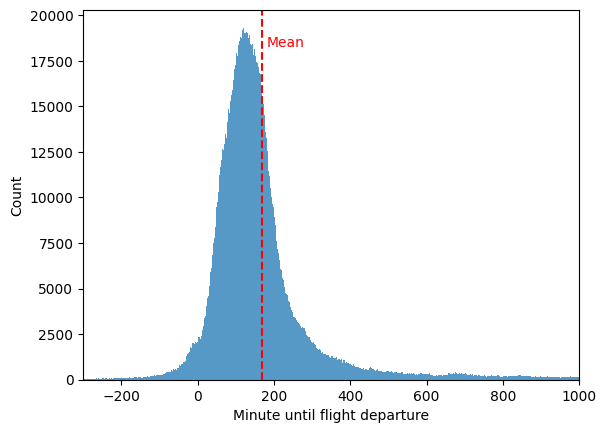
\includegraphics[width=0.6\textwidth]{Minute until flight departure.png}\\
    \caption{Minute until flight departure distribution}
    \label{fig:Minute until flight departure distribution}
\end{figure}
\FloatBarrier

\FloatBarrier
\begin{figure}[ht]
  \centering
  \begin{subfigure}{0.48\textwidth}
    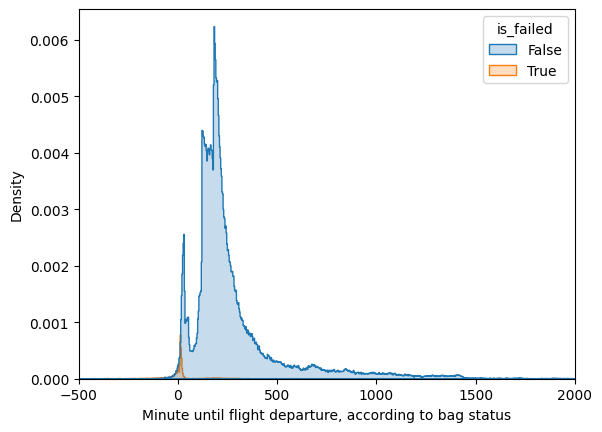
\includegraphics[width=\linewidth]{Minute until flight departure_2.png}
    \caption{Macro view}
  \end{subfigure}
  \hfill
  \begin{subfigure}{0.48\textwidth}
    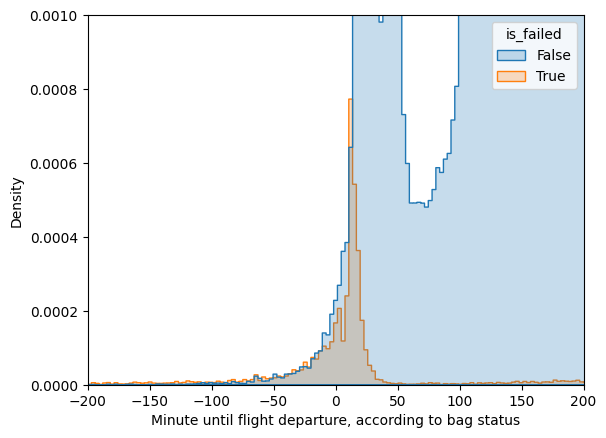
\includegraphics[width=\linewidth]{Minute until flight departure_3.png}
    \caption{Micro view}
  \end{subfigure}
  \caption{Minute until flight departure distribution according to bag status}
  \label{fig:Minute until flight departure distribution according to bag status}
\end{figure}


\subsubsection{Geographical links}

\noindent Pretty late during the year, I accessed the flights informations of each bag paths data. This dataset concerns only transiting bags\footnote{Bags arriving at CDG airport by an inbound flight in the aim to be loaded in an outbound fight with another destination. Those bags doesn't exit at CDG and are pushed in the \acrshort{bhs} at their arrival.}. Those data gave us additional informations, and the most relevant were geographical origins and destinations. They are key informations in the logistic for two reasons. 
\begin{itemize}
    \item \textit{Ball baggage} : One of the baggage hazards that can delay a bag journey in the \acrshort{bhs} process is when bag falls off a conveyor belt. When this happens, a handler is called in and has to walk to the location to put the baggage back on the conveyor belt. The handlers have noted that the concerned type of baggage are very often ball baggage, which as the name suggests, are baggage in the shape of a ball (or rounded bags). Because of this shape, they are more likely to roll and fall off the facilities. Finally, although we don't have any statistics on this type of baggage, handlers have pointed out that very often, the origin or destination of the ball bags are African country. For these reasons, including the origin and destination of a piece of baggage can make it possible to include an additional difficulty linked to the type of baggage.


    \item \textit{Parking areas} : The second impact of origin and destination is the flight parking areas. As flight companies share terminal and check in doors, they also share parking areas. We don't have exact plans of it, but as the airport is extremely large, the destination and origins of flights could add geographical information within the airport in the model. For example, if a bag comes from an european country and is going to another european country, it is more likely that it uses the same company for both flights. Therefore, the path and process in between its arrival and departure would be shorter. On the other hand, a bag coming from Ireland and taking a flight for China will probably not use the same company. So the parking areas might be more far away from each other.

\end{itemize}


\noindent For the locations, even tho we had precised data like name of airports and countries, I decided to use continent only to reduce the complexity of models and avoid unnecessary noise. 

\noindent The figure bellow is the heat-map of percentage of failed bags according to their origins and destinations.

\noindent I also computed the heat-map for the time duration according to geographical links.


\noindent To encode those data, I grouped each possible origins and destinations links possible. As we are interested by the links effect (for example a bag from Africa and going to America), it would be more efficient for models to have one column for links (\textit{from Africa to America}) instead of two separated columns for origin and destination. Finally, as those are categorical data I encoded them with the one-hot encoder strategy.

Mettre les tables pour les noms de données encodées


%\subsubsection{Maintenance operations}

%\subsection{Stored bags}

\newpage
\section{Imbalanced dataset issue}\label{section:Imbalanced dataset issue}

\subsection{Confusion matrix and metrics}

The question of unbalanced datasets is one of the interesting issues to deal with in machine learning. In a classification, we want to predict which of the different possible events will occur. To train an algorithm, it needs a certain amount of data in order to calibrate its coefficients with the training dataset, and test the best theoretical coefficients with the test dataset. During classification, the different classes may not be equally distributed. 
\cite{ArtificialIntelligenceReview}

\begin{figure}[htbp]
    \centering
    \begin{minipage}{0.55\textwidth}
        \centering
        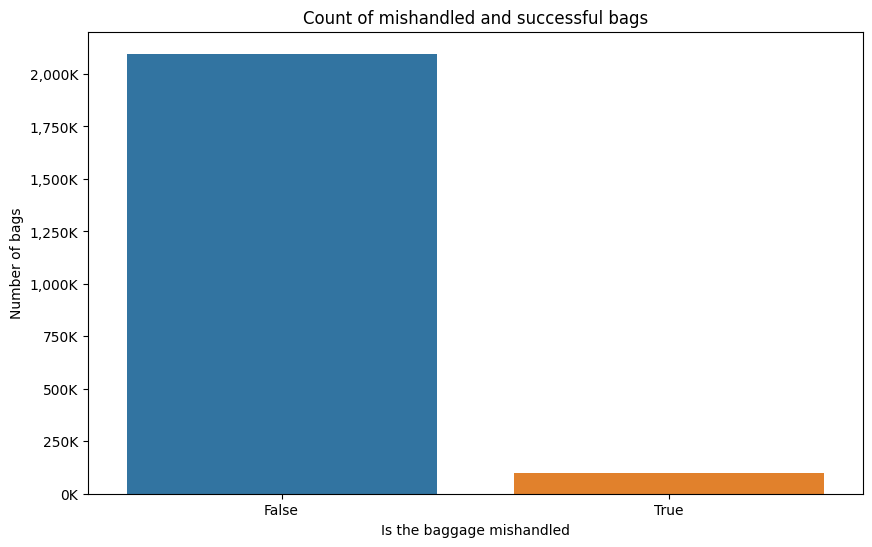
\includegraphics[width=\textwidth]{is_failed unbalanced.png} % Replace 'example-image' with your image file
        \caption{Proportion difference of failed and non-failed bag}
        \label{fig:Proportion difference of failed and non-failed bag}
    \end{minipage}
    \hfill
    \begin{minipage}{0.3\textwidth}
        In our case of failed baggage, the \autoref{fig:Proportion difference of failed and non-failed bag} shows the difference between the number of non-failed and failed bags. Fortunately for passengers, the number of failed bags is far smaller than the number of non-failed bags. In our dataset, there are 4 failed bags for every 100 non-failed bags.
    \end{minipage}
\end{figure}

AJOUTER REFERENCE POUR LE PROBLEME DE SURAPPRENTISSAGE EN IMBALANCED DATASET

This large difference in proportions is problematic, because when training the models, there's a risk of over-training them to predict non-missed baggage. Indeed, if 95\% of baggage is not missed, the models will be able to get a good score by predicting 100\% of non-missed baggage. However, there is a risk of not being able to predict missed baggage. To overcome this problem, we first take a look at the confusion matrix. Having a look at the \autoref{tab:Confusion Matrix}, we can try to understand the confusion matrix concept. 
\begin{table}[htbp]
    \centering
    \captionsetup{justification=centering}
    \caption{Confusion Matrix}
    \label{tab:Confusion Matrix}
    \newcommand{\cellcolorpos}{\cellcolor{cyan!20}}
    \newcommand{\cellcolorneg}{\cellcolor{yellow!20}}
    \begin{tabular}{cc|c|c|}
        \cline{3-4}
        & & \multicolumn{2}{c|}{\textbf{Actual}} \\
        \cline{3-4}
        & & \textbf{Positive} & \textbf{Negative} \\
        \hline
        \multicolumn{1}{|c|}{\multirow{2}{*}{\textbf{Predicted}}}
        & \textbf{Positive} & \cellcolorpos True Positive (TP) & \cellcolorneg False Positive (FP) \\
        \cline{2-4}
        \multicolumn{1}{|c|}{}
        & \textbf{Negative} & \cellcolorneg False Negative (FN) & \cellcolorpos True Negative (TN) \\
        \hline
    \end{tabular}
\end{table}
\noindent This matrix gives four different informations : 
\begin{itemize}
\centering
    \item \textbf{TP} : The model predicted a \textit{True} event while it was actually \textit{True}.
    \item \textbf{TN} : The model predicted a \textit{False} event while it was actually \textit{False}.
    \item \textbf{FP} : The model predicted a \textit{False} event while it was actually \textit{True}.
    \item \textbf{FN} : The model predicted a \textit{True} event while it was actually \textit{False}.
\end{itemize}

Therefore in the context of failed baggage issue, we might manage to predict a high number of non-failed bags (FP will be high) but struggle to predict failed bags as it is the minority class (TP will be lower). 
Having a look at some metrics might help to understand the problem and how to manage it.
The accuracy compute the ratio of good predictions over all the population. It doesn't mind if one of the class got a bad prediction score. Using this metric only can lead to over estimate the capacity of the model. If the model predict 100\% of the bags as non-failed, as it is the majority class, the accuracy might be very high even thought the number of TP is null. 
\begin{equation}
\text{Accuracy} = \frac{\sum{TP + TN}}{\sum{TP + TN + FP + FN}}    
\end{equation}

The recall compute the ratio of TP over the TP and the FN populations. Having a high recall rate means we didn't predict much actually positive status as negative one. In the bags issue, it means we would not predict failed bags as non-failed. Reversely, having a low recall means we predict too much failed bags as being non-failed. This ratio will be very important as it will give information on the ability of the model to predict failed-bags.
\begin{equation}\label{equation:Recall}
\text{Recall} = \frac{\sum{TP}}{\sum{TP + FN}}    
\end{equation}

The precision is the ratio of TP over TP and FP populations. It measures how many of the predicted positive instances are actually positive. A high precision indicates that when the model predicts positive values, it is actually correct (So we have a lower number of FP).

\begin{equation}\label{equation:Precision}
\text{Precision} = \frac{\sum{TP}}{\sum{TP + FP}}
\end{equation}

Both recall and precision are important to optimise a model, especially when to target classes are imbalanced. However, deciding to optimise the recall to predict the maximum of failed-bags would also increase the number of false positive (non-failed bags predicted as failed). Reversely, optimising the model by maximising the precision would increase the false negative, meaning that more failed-bags wont be predicted. 
To find the best trade-off between precision and recall, the F1-score combines both metrics. A high F1-score coefficient indicates that both recall and precision are quite good. In such a case, we can consider the model as accurate for positive predictions. In the case of imbalanced dataset, the F1-score will give more balanced measured by considering both precision and recall. 
\begin{equation}\label{equation:F1-score}
\text{F1-Score} = 2 \cdot \frac{\text{Precision} \cdot \text{Recall}}{\text{Precision} + \text{Recall}}    
\end{equation}

\newcommand{\mycomment}[1]{}

\mycomment{

\subsection{Concept of class weights}

\noindent Class weights are coefficients assigned to classes in order to handle imbalanced datasets. When data is imbalanced, the class with the majority of instances can dominate the learning process, causing the model to perform poorly on the minority class. By assigning higher weights to minority classes and lower weights to majority classes, the model can be made more sensitive to the minority class, improving overall performance. For imbalanced datasets, class weights adjust the learning algorithm to pay more attention and give more power to the minority class, helping to balance the model's performance across all classes.
 
\noindent In a \textbf{logistic regression}, class weights are incorporated into the loss function (\cite{AppliedMachineLearning}). The weighted loss function is then given by :
\begin{equation}
L(\theta) = -\sum_{i=1}^{n} w_i \left[ y_i \log(p_i) + (1 - y_i) \log(1 - p_i) \right]
\end{equation}
 
where \( w_i \) are the class weights, \( y_i \) are the true labels, and \( p_i \) are the predicted probabilities.
 
In \textbf{Random Forest}, class weights can be applied to the criterion used to split the nodes. The Gini impurity or entropy can be weighted by the class weights. For instance, the weighted Gini impurity is:
 
\begin{equation}
G_w = \sum_{k=1}^{K} w_k p_k (1 - p_k)
\end{equation}
 
where \( w_k \) is the weight for class \( k \), and \( p_k \) is the proportion of class \( k \) at a given node.
 
For Gradient Boosting algorithms like \textbf{XGBoost} and \textbf{LightGBM}, class weights can be used to scale the gradients and Hessians during the boosting process. The weight-adjusted loss function for gradient boosting algorithm can be represented as:
 
\begin{equation}
L(\theta) = \sum_{i=1}^{n} w_i \ell(y_i, f(x_i))
\end{equation}
 
where \( \ell \) is the loss function, \( w_i \) are the class weights, \( y_i \) are the true labels, and \( f(x_i) \) are the model predictions.
 
In LightGBM, class weights adjust the gradient and Hessian as follows:
 
\begin{equation}
g_i = w_{y_i} \frac{\partial \ell(y_i, f(x_i))}{\partial f(x_i)}
\end{equation}
 
\begin{equation}
h_i = w_{y_i} \frac{\partial^2 \ell(y_i, f(x_i))}{\partial f(x_i)^2}
\end{equation}
 
where \( g_i \) and \( h_i \) are the gradient and Hessian for the \( i \)-th sample, respectively.


}


\newpage
\subsection{Under-sampling}
%\subsection{SMOTE : Synthetic Minority Over-sampling Technique}



\newpage
\section{Models}
% introduction sur le choix des modèles


%\subsubsection{Hyper-parameter optimisation}
\newpage 
\subsection{Logistic regression}\label{subsec:Logistic regression}


\newpage
\subsection{\acrlong{rf}}



\newpage
\subsection{Light Gradient Boosting Machine}
\acrlong{lgbm} (developped by \cite{LightGBM}) is another popular gradient boosting framework designed to be highly efficient and scalable. It is particularly well-suited for handling large-scale data and offers several advantages over traditional gradient boosting methods.
 
LightGBM uses a histogram-based approach for constructing decision trees, which significantly reduces memory usage and improves training speed. It also includes several optimization techniques that enhance its performance and generalization capabilities.
 
Key features of LightGBM include:
 
\begin{itemize}
    \item Gradient-based One-Side Sampling (GOSS): LightGBM uses GOSS to filter out data instances with small gradients, focusing on the instances with larger gradients that have a greater impact on the model. This reduces the data size without compromising accuracy.
    \item Exclusive Feature Bundling (EFB): EFB reduces the number of features by bundling mutually exclusive features together, which minimizes memory consumption and speeds up training.
    \item Leaf-wise Tree Growth: Unlike other gradient boosting methods that use level-wise tree growth, LightGBM grows trees leaf-wise. This means it splits the leaf with the maximum loss reduction, leading to deeper trees and better accuracy.
\end{itemize}
 
The LightGBM algorithm can be summarized in the following steps:
 
\begin{algorithm}[H]
\caption{LightGBM Algorithm}
\begin{algorithmic}[1]
    \State \textbf{Input:} Training data $(x_i, y_i)$, number of iterations $M$, learning rate $\eta$
    \State \textbf{Initialize:} $f_0(x) = \log\left(\frac{\bar{y}}{1 - \bar{y}}\right)$
    \For{$m = 1$ to $M$}
        \State Compute the gradients and hessians: $g_{im} = \frac{\partial L(y_i, \hat{y}_i^{(m-1)})}{\partial \hat{y}_i^{(m-1)}}$, $h_{im} = \frac{\partial^2 L(y_i, \hat{y}_i^{(m-1)})}{\partial (\hat{y}_i^{(m-1)})^2}$
        \State Perform histogram-based binning of features.
        \State Apply GOSS to select a subset of instances.
        \State Construct a decision tree using the selected instances and EFB.
        \State Update the model: $f_m(x) = f_{m-1}(x) + \eta h_m(x)$
    \EndFor
    \State \textbf{Output:} Final model $f_M(x) = f_0(x) + \sum_{m=1}^{M} \eta h_m(x)$
\end{algorithmic}
\end{algorithm}
 

\noindent LightGBM optimizes the same objective function as the XGBoost (see \autoref{equa:Gradient Boosting objective function}). LightGBM's effectiveness and efficiency make it a powerful tool for many machine learning tasks, particularly when dealing with large and complex datasets.

\newpage
\subsection{Probability calibration}

\subsubsection{Platt Scaling}\label{Platt scaling}
 
Platt scaling is a method for transforming the output of a binary classifier into a probability score. It involves fitting a logistic regression model to the classifier scores. The logistic regression model is trained using the classifier scores as input and the true binary labels as the target. The formula for Platt scaling is given by:
 
\begin{equation}
P(y=1|x) = \frac{1}{1 + \exp(Af(x) + B)}    
\end{equation}

 
where \( f(x) \) is the output of the classifier for input \( x \), and \( A \) and \( B \) are parameters learned from the training data.
 
\subsubsection{Isotonic Regression}\label{Isotonic regression}



ref : \cite{JasonBrownlee} \& \cite{ExperianLatAmDataLab}


\newpage
\section{Training Methodology}
\subsection{Data normalisation}
Explain choice of Robust Scaler
\subsection{Data splitting}
\subsection{Cross validation}
explication KFold stratified cross validation, 

\subsection{Hyper parameters optimization}




\newpage
\section{Results}

La \autoref{tab:List of models} recense les résultats de chaque modèle. Pour chaque modèle, le F1-Score ainsi que l'average precision (AP) ont été calculé avec leur seuil de classification optimal. 
Le modèle 1, la regression logistique servant de référence est le modèle avec la plus faible qualité de classification. Cela montre que la classification est assez complèxe est qu'il est alors utile d'utiliser des modèles de machine learning plus poussés.


\paragraph{Plot metrics}


Faire une table logistic reg, lgbm, plat scaling, isotonic


\section{Agnostic methods}


\newpage
\section*{Conclusion}
\addcontentsline{toc}{section}{Conclusion}

\newpage
\section*{Appendix}
\addcontentsline{toc}{section}{Appendix}

\subsection*{Graphics and tables of models results}
\addcontentsline{toc}{subsection}{Graphics and tables of models results}

\newpage
\FloatBarrier
\begin{table}[ht]
\centering
\caption{List of models}
\label{tab:List of models}
\renewcommand{\arraystretch}{3}
\begin{small}
\begin{tabularx}{\textwidth}{|c|X|X|c|c|c|}
\hline
\textbf{ID} & \textbf{Name} & \textbf{Description} & \textbf{Threshold} & \textbf{F1-Score} & \textbf{AVP} \\ \hline
1 & Logistic regression & Main features & 0.5 & test & test \\ \hline
2 & RF & Main features & 0.5 & test & test \\ \hline
3 & LGBM & Main features & 0.5 & test & test \\ \hline
4 & Logistic regression & Path duration with noise added & 0.5 & test & test \\ \hline
5 & RF & Path duration with noise added & 0.5 & test & test \\ \hline
6 & LGBM & Path duration with noise added & 0.5 & test & test \\ \hline
7 & LGBM & Random search optimization & 0.5 & test & test \\ \hline
8 & LGBM + Platt scaling & Platt scaling for probability calibration & 0.5 & test & test \\ \hline
9 & LGBM + Isotonic regression & Isotonic regression for probability calibration & 0.5 & test & test \\ \hline
10 & LGBM + undersampling & Undersampling method & 0.5 & test & test \\ \hline
\end{tabularx}
\end{small}
\end{table}
 
\FloatBarrier



\newpage
\subsubsection*{Model 1}
\addcontentsline{toc}{subsubsection}{Model 1}
\textbf{Logistic regression}



\newpage
\textbf{\acrlong{rf} without path duration}

\FloatBarrier
\begin{figure}[ht]
  \centering
  \begin{subfigure}{0.41\textwidth}
    \includegraphics[width=\linewidth]{rf 1 probability distribution.png}
  \end{subfigure}
  \hfill
  \begin{subfigure}{0.41\textwidth}
    \includegraphics[width=\linewidth]{rf 1 classification report seuil.png}
  \end{subfigure}
  \caption{Random Forest without calibration results (without path duration)}
  \label{fig:Random Forest uncalibrated (without path duration)}
\end{figure}
\FloatBarrier









\newpage
\textbf{\acrshort{lgbm} without path duration}


\newpage
\subsubsection*{Models with path duration with noise}
\addcontentsline{toc}{subsubsection}{Models with path duration with noise}

\newpage
\subsection*{Other graphics}
\addcontentsline{toc}{subsection}{Other graphics}

\begin{figure}[h]
    \centering
    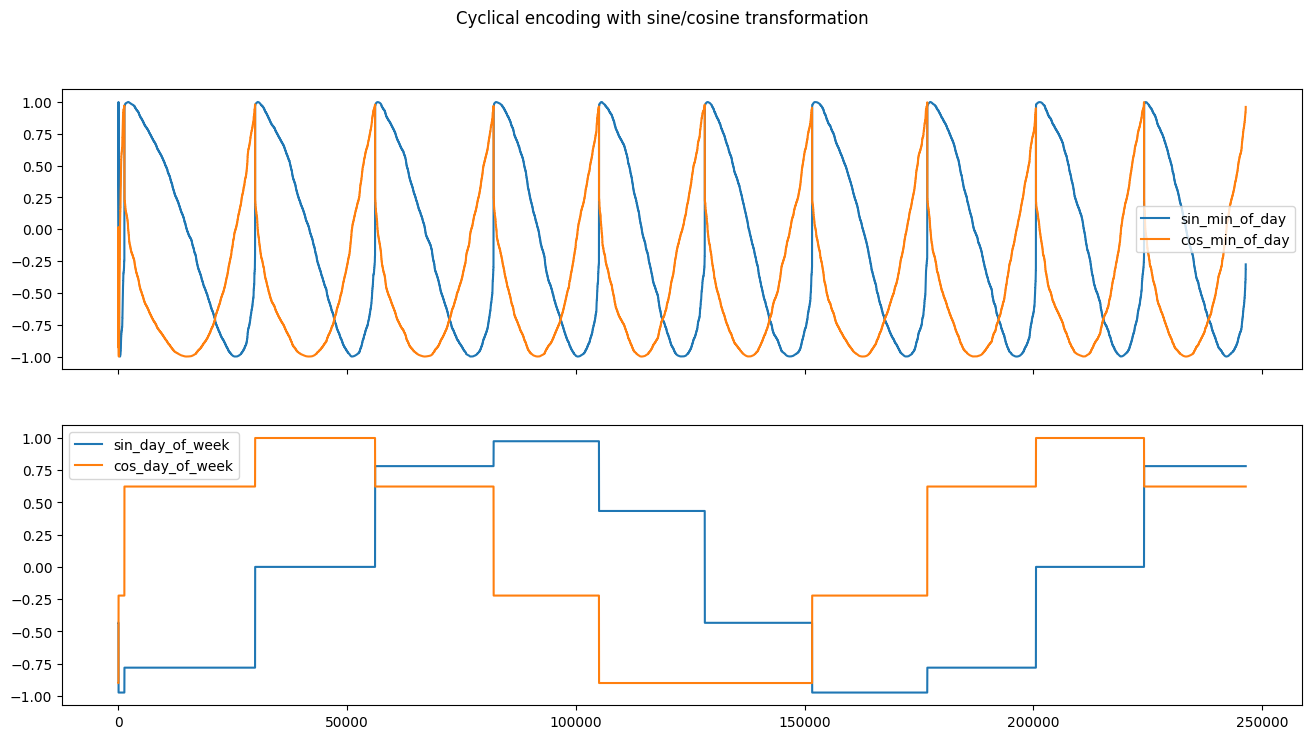
\includegraphics[width=0.9\textwidth]{cyclical encoding.png}\\
    \caption{Cyclical encoding of days and minutes}
    \label{fig:Cyclical encoding of days and minutes}
\end{figure}
\FloatBarrier

\newpage
\printglossaries



\newpage
\printbibliography




\end{document}
